% !Mode:: "TeX:UTF-8"
\chapter{研究背景与意义}
\label{cha:intro}

\section{研究背景}
\label{sec:background}

随着智能制造、服务机器人以及自动驾驶技术的飞速发展，具备高精度环境感知与自主交互能力的智能系统正成为学术界与工业界的研究焦点。在这一领域中，三维点云（3D Point Clouds）凭借其对物体几何结构和空间尺度的精确表达能力，已成为连接物理世界与数字世界的重要纽带。作为一种无序、非结构化的数据集合，点云能够直接反映物体的真实拓扑结构，不存在二维图像中的透视形变，因此被广泛应用于逆向工程、三维重建、场景理解以及机器人自主抓取等关键任务中~\cite{mirzaei_3d_2022}。

在点云数据分析中，物体几何特征（尤其是边缘与角点）的提取不仅是数据简化的过程，更是语义理解的关键。边缘勾勒了物体的轮廓骨架，角点则确立了形体的关键节点。这些特征承载了最丰富的结构语义信息：在三维重建中，它们往往作为曲面拟合的自然边界，决定了重建模型的保真度~\cite{li_surface_2023}；在物体识别与配准任务中，它们充当了具有高辨识度的关键描述符，能够显著提升算法在复杂场景下的鲁棒性~\cite{lavin-delgado_efficient_2024, GaoJunJie_ji_2024, ZhangZhiJia_ji_2017}；而在机器人操作领域，准确的轮廓信息更是实现精细化装配与灵巧抓取的前提条件~\cite{ahmed_edge_2018}。

尽管物体几何特征具有重要的应用价值，但从非结构化点云中自动且精确地检测这些特征仍面临严峻挑战。首先受限于物理平滑及采样精度，现实物体原本的尖锐几何特征在点云数据中往往表现为一定范围内的圆角过渡区域，使得边缘和角点的界定变得模糊，不利于检测。其次是不同类别的几何特征数据分布的极度不平衡。在一个完整的物体点云中，绝大多数点属于平坦表面，边缘点次之，而角点最为稀疏。
传统上，局部几何描述符（如协方差矩阵的特征值~\cite{gumhold_feature_2001}、法向量~\cite{demarsin_detection_2007}和曲率~\cite{nguyen_edge_2018}）通常被用于提取边缘和角点，但这些方法依赖于人工调整的参数和阈值。其优势在于简单且计算效率高，却往往受困于难以调整的阈值、模糊的特征界定以及变化的尺度，难以兼顾检测的灵敏度与特异性。

另一方面，基于学习的方法有潜力解决上述部分缺陷。训练好的模型无需调整参数和阈值~\cite{charles_pointnet_2017a, bazazian_edcnet_2021}即可实现检测，表现出优越的适应性和鲁棒性。边缘特征提取已被广泛研究~\cite{himeur_pcednet_2022, bode_bounded_2023}，这些方法利用网络学习从局部解析特征到几何特征的映射，在边缘检测方面表现出色。然而，现有的数据驱动方法往往忽略了角点检测，或因缺乏针对性设计而导致角点检测精度低。角点检测面临着诸如与边缘特征相似、数据可用性有限以及对尺度更敏感等特有问题。这些问题在专门针对角点检测的方法~\cite{wang_pienet_2020}中也依然存在，常表现为较高的误报率和特征点的误分类。

在机器人物理交互层面，机器人抓取规划（Robotic Grasp Planning）是实现自主操作的核心环节，其生成的目标物体抓取构型对于规划操作任务中的机器人运动至关重要~\cite{li_survey_2019}。传统的机器人系统往往依赖于耗时费力的人工示教，而近年来广泛研究的自动化抓取规划算法~\cite{newbury_deep_2023}，极大地推动了自主操作技术的发展。

机器人抓取规划的核心目标是生成既满足力学稳定性又具备空间灵活性的抓取候选。早期的研究为解析抓取方法奠定了理论框架基础~\cite{asada_studies_1979}。研究人员利用图元拟合~\cite{miller_automatic_2003, goldfeder_grasp_2007}或表面分割~\cite{harada_grasp_2011, wan_planning_2021}等技术开发了基于已知模型的规划算法。这些解析方法不仅通过模型匹配支撑了装配、分拣等在线操作任务~\cite{chen_category_2022}，也为构建离线数据库以训练端到端的抓取规划器提供了数据基础。

目前的抓取规划算法主要强调面接触的重要性，以确保抓取的鲁棒性。这种倾向同样存在于端到端的学习方法中，因为它们通常在以面接触为核心的数据集~\cite{mahler_dexnet_2017, lenz_deep_2015}上进行训练。面接触策略通过将手爪指腹与物体表面法线对齐来实现最大化接触面积，虽然能提供稳定的抓取，但往往以牺牲灵活性为代价。在处理复杂多面体、非对称形状或具有丰富锐角结构的物体时，这种刚性约束常会导致规划失败。尽管部分研究试图通过设计特殊的指尖~\cite{song_fingertip_2018, ringwald_towards_2023}或利用多指手爪~\cite{grady_contactopt_2021}来增加接触面积，但面接触优先策略仍限制了抓取策略对广泛物体形状的适应能力。

边缘和角点通常因被认为不稳定而被排除在抓取采样之外。在刚体接触假设下，边缘或角点上的接触退化为点接触，抗扭矩能力有限~\cite{bicchi_robotic_2000}。然而，在引入软接触（Soft Contact）模型后，指腹的弹性形变可以包裹住尖锐特征，从而有效地模拟面接触。这一范式的转变使得涉及边缘和角点的抓取成为可能，不仅增强了抓取的灵巧性，还将其适用性扩展到了面接触优先规划器无法触及的复杂物体上。

基于上述背景，本文的研究动机源于两个紧密耦合的需求：一是如何从非结构化点云中提取出高保真的几何结构信息，实现对面、边缘及角点的高精度同步检测，解决稀疏角点特征难识别的问题；二是如何利用这些检测到的丰富几何特征，突破面接触的局限，规划出更灵活、更多样、覆盖率更高的机器人抓取构型。本文致力于构建一套完整的从几何感知到抓取规划的技术框架，以解决当前特征检测精度不足和抓取策略灵活性受限的关键问题。


\section{国内外研究现状}
\label{sec:related_work}
针对基于点云信息的物体几何特征检测和机器人抓取规划两个研究领域，国内外学者已经开展了大量研究工作。本章节将对这两个领域的研究现状进行详细综述，重点分析现有方法的技术路线以及优缺点。
\subsection{物体几何特征检测研究现状}
针对点云数据的物体几何特征检测旨在从无序点云中区分出具有语义信息的结构特征，可以区分为平滑特征（平滑面）和尖锐特征（边缘、边界及角点）两大类。根据技术路线的不同，现有方法主要分为传统的解析方法和基于深度学习的数据驱动方法。

\subsubsection{传统解析方法}
传统方法包括基于人工设计的几何描述符、基于表面网格重建以及基于图的方法以及来表征局部邻域的统计特性等，实现不同几何特征的区分。其中基于人工设计的几何描述符是最早被广泛研究的技术路线。

Gumhold等人~\cite{gumhold_feature_2001} 提出的基于主成分分析（PCA）的方法是该领域的经典工作。该方法通过构建点云中每个点及其 $k$ 近邻点的协方差矩阵，计算该矩阵的特征值来描述局部表面的几何变化。如图~\ref{fig:gumhold_feature_2001} 所示，不同几何特征的邻域范围内存在不同的数据分布。具体而言，如果不为零的最小特征值超过了预设的阈值，则认为该点附件的数据变化程度较大，属于边缘或角点特征。
\begin{figure}[htbp]
    \centering
    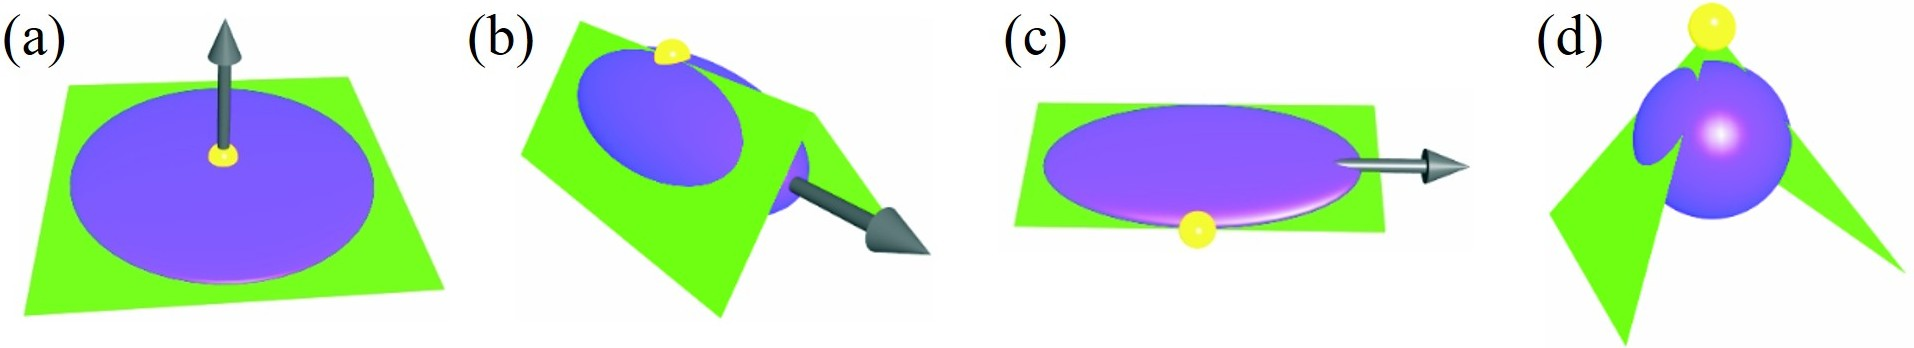
\includegraphics[width=0.85\textwidth]{Others/gumhold_feature_2001.jpg}
    \bicaption{不同几何特征点的邻域形状~\cite{gumhold_feature_2001}：(a) 平面点；(b) 折边点；(c) 边界点；(d) 角点。}{Neighborhood shapes of different geometric feature points~\cite{gumhold_feature_2001}: (a) Face point; (b) Ridge point; (c) Boundary point; (d) Corner point.}
    \label{fig:gumhold_feature_2001}
\end{figure}

在 PCA 方法的基础上，Xia等人~\cite{xia_fast_2017} 进一步引入了基于局部协方差矩阵的特征值比率的边缘检测算法，通过分析特征值之间的相对关系，实现几何特征的检测。Pauly等人~\cite{pauly_multiscale_2003} 和 Bazazian等人~\cite{bazazian_fast_2015} 则提出了多尺度分析框架，通过综合不同邻域尺度下的几何响应值来增强特征检测的鲁棒性。多尺度分析能够在一定程度上缓解单一尺度选择带来的问题，但仍然依赖于人工设定的阈值，且在处理具有复杂几何结构的物体时，特征点的界定仍然模糊不清。

Nguyen等人~\cite{nguyen_edge_2018} 基于曲率进行边缘特征提取并分为三个阶段：先利用曲率估计并配合阈值策略定位可能的边缘点；再通过迭代非极大值抑制对高曲率响应的宽带区域进行压缩与精炼，以获得更准确、稀疏的边缘点集合；最后基于距离阈值判定点与点之间的邻接关系，将相邻点逐步连接形成连续的特征线或边缘，从而实现稳定的线状特征恢复。王丽辉等人~\cite{WangLiHui_san_2011} 则结合曲率和法线信息进行邻域分析，并通过八叉树结构计算模型数据点密度，利用密度信息辅助边缘点的提取和连接，提升了边缘检测的准确性和连续性。

基于图的方法可以通过结合全局上下文信息进一步增强特征提取。例如，Demarsin等人~\cite{demarsin_detection_2007} 针对曲线的检测开展相关工作。其先基于点云法线信息，通过一阶分割获得候选特征点，并将其组织为图结构以恢复锐特征线；随后构建最小生成树以形成初始线结构，并通过后续的重连接过程将断裂的线段闭合，从而获得闭合特征线。此外，Che等人~\cite{che_multiscan_2018} 采样了一种无需通用法向估计的方法：首先设计了新的特征提取策略 NORmal VAriation ANAlysis（Norvana），能够剔除部分噪声点并提取边缘点；随后采用区域生长，将同一平滑曲面上的点聚合得到分割结果。图~\ref{fig:che_multiscan_2018} 展示了Norvana的结构。
\begin{figure}[htbp]
    \centering
    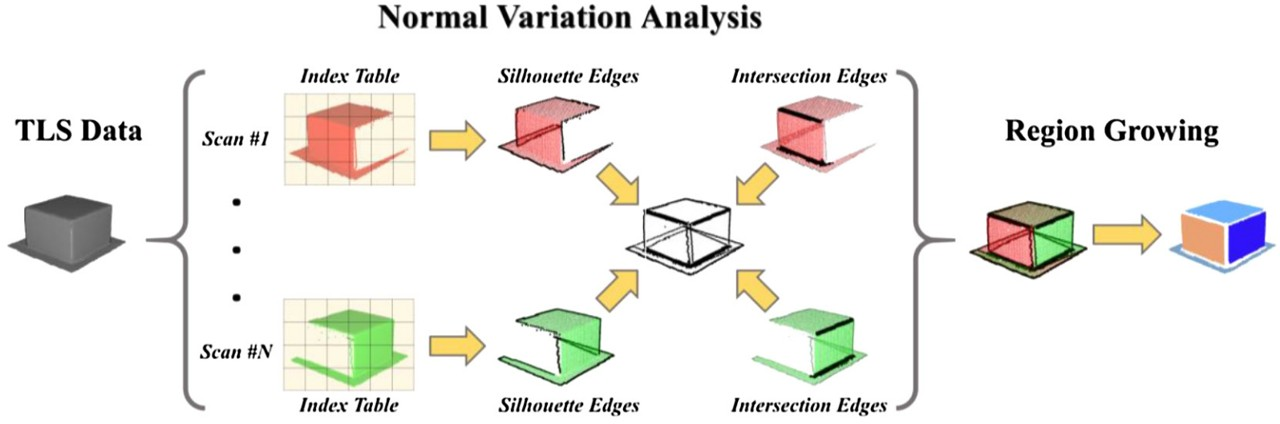
\includegraphics[width=0.85\textwidth]{Others/che_multiscan_2018.jpg}
    \bicaption{基于法向量分析的边缘检测方法Norvana~\cite{che_multiscan_2018}。}{Norvana: Normal Variation Analysis-based edge detection method~\cite{che_multiscan_2018}.}
    \label{fig:che_multiscan_2018}
\end{figure}

基于表面重建的方法，如利用移动最小二乘法（Moving Least Squares, MLS）~\cite{daniels_robust_2007}，可以通过利用局部近似来改善尖锐特征的检测。该方法首先在局部邻域内拟合一个高阶多项式曲面，然后分析数据点到拟合曲面的残差分布。特征点通常表现为拟合残差较大的区域，或者拟合曲面曲率极大的位置。这类方法的优势在于能够提供亚像素级别的特征定位精度，但高阶曲面拟合的计算开销较大，且在特征交汇复杂的角点区域容易产生伪影。Zhang等人~\cite{zhang_multinormal_2019} 提出了 VAM，利用成对一致性投票机制进行法向量估计，在尖锐边缘或角点处允许存在多个法向量假设，并通过邻域内的一致性投票来筛选出最能代表几何结构的法向量组合，从而有效地在重建过程中保留尖锐特征。

Lin等人~\cite{lin_line_2015} 则利用多视图投影点云的方法进行边缘检测。如图~\ref{fig:lin_line_2015} ，其将三维点云进行多视图投影，再基于二维图像的线段检测算法（LSD）进行边缘提取，最后将检测到的线段重新映射回三维空间。并利用半平面线段分割结构（Line-Segment-Half-Planes, LSHP）进行进一步的匹配，得到完整的三维线段特征。该方法通过引入多视图投影的策略，成功地将二维图像处理技术应用于三维点云的边缘检测中。
\begin{figure}[htbp]
    \centering
    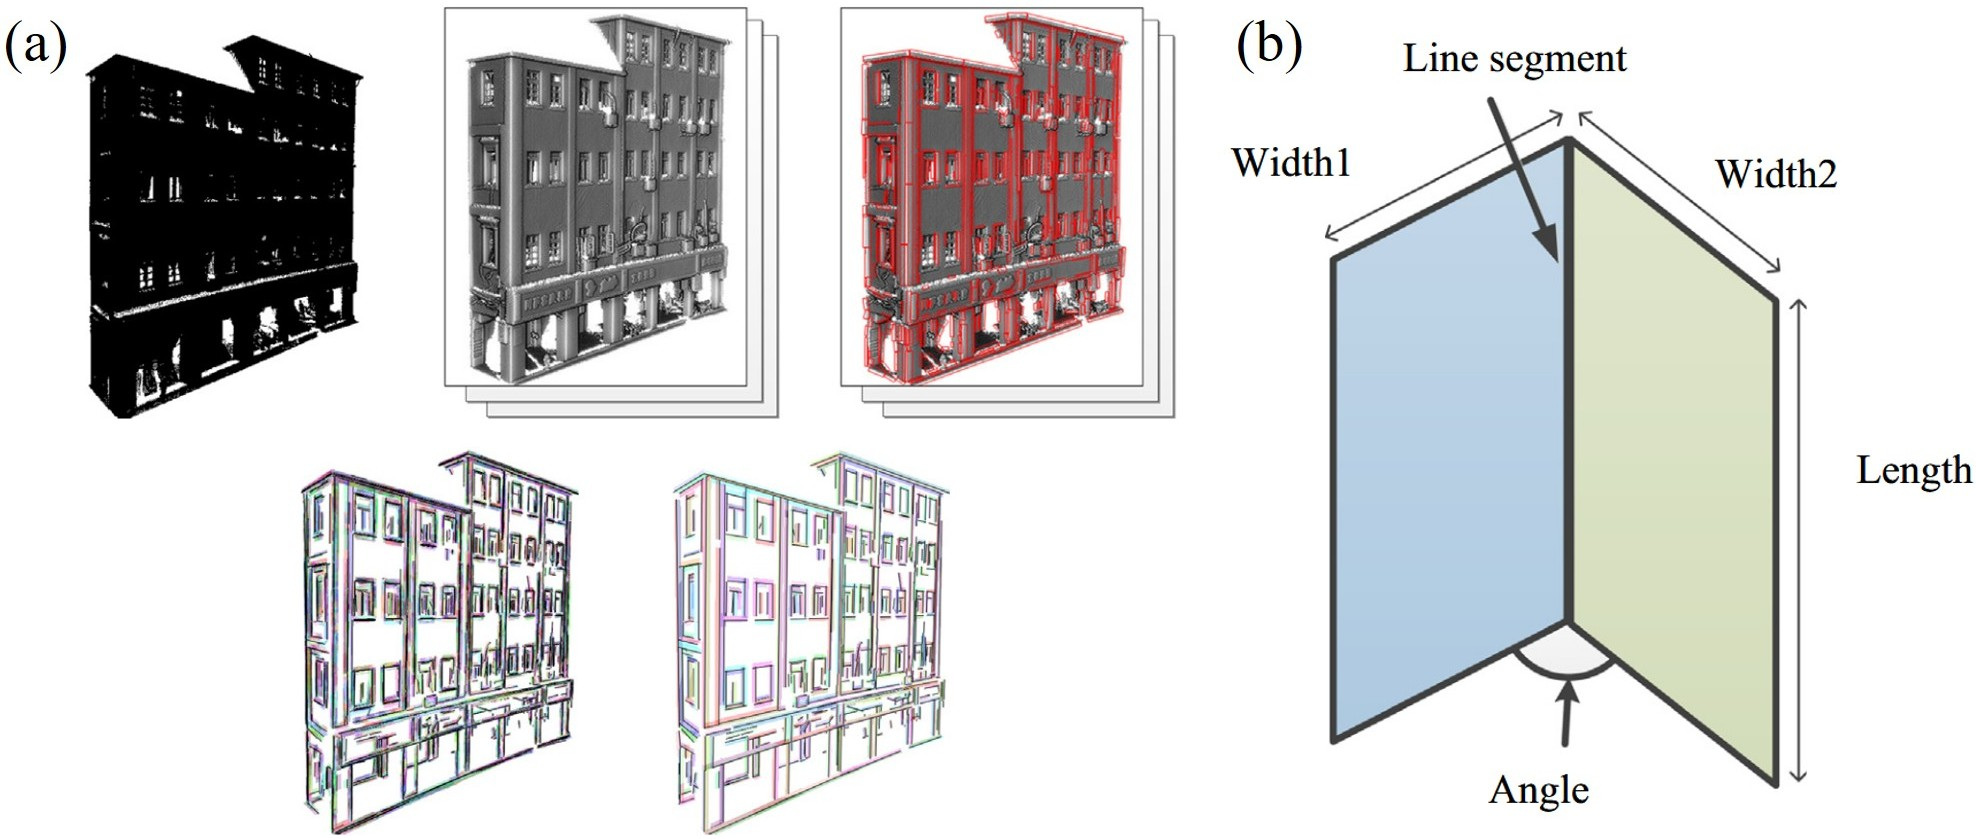
\includegraphics[width=0.85\textwidth]{Others/lin_line_2015.jpg}
    \bicaption{基于多视图投影的三维点云边缘检测流程~\cite{lin_line_2015}：(a) 各阶段检测结果；(b) LSHP结构示意图。}{Multi-view projection-based 3D point cloud edge detection pipeline~\cite{lin_line_2015}: (a) The detection results of each stage; (b) Schematic of the LSHP structure.}
    \label{fig:lin_line_2015}
\end{figure}

在角点检测方面，针对仅提取边缘不足以描述完整几何特征的问题，Ahmed等人~\cite{ahmed_edge_2018} 采用了两步提取过程：首先基于邻域的空间分析区分出面点和非面点，然后利用聚类的方法在非面点中识别角点。此外，Schmidt等人~\cite{schmidt_detection_2023} 提出使用 RANSAC 算法从点云中提取直线或平面，并在它们的交点处检测角点。这些方法尝试通过几何基元的组合关系来定位角点，但在复杂噪声环境下仍面临挑战。

综上所述，虽然以几何描述符、表面重建及图优化为代表的传统解析方法为点云特征提取奠定了理论基础，并在规则模型的边缘检测中表现出一定有效性，但其局限性亦十分显著。首先，这类方法本质上依赖于人工设计的几何规则与先验假设，对噪声极其敏感，且高度依赖如邻域尺度、曲率阈值等参数的精细调节，难以在物体形状多变、数据质量参差的现实场景中实现自适应的稳健检测。其次，基于平滑拟合的策略往往导致尖锐特征被过度平滑，造成定位精度损失。最为关键的是，角点检测在此类方法中常被边缘化，多作为边缘提取后的二次处理步骤或依赖于理想化的平面相交假设，这种两阶段策略不仅计算冗余，且在处理复杂拓扑结构的角点时极易因特征模糊而产生误检或漏检。

\subsubsection{基于数据驱动的方法}
近年来，随着深度学习在三维视觉领域的突破，基于数据驱动的几何特征检测方法逐渐成为主流。这类方法通常将特征提取任务建模为分类或回归问题，将点云中的每个点标记为属于特定的几何类别或找出拟合的几何参数。相较于传统方法，数据驱动模型不再依赖人工设定的复杂阈值，而是通过神经网络自动学习从局部几何结构到特征类别的映射关系，展现出更强的鲁棒性和泛化能力。

点云数据存在无序、稀疏且高维的特点，传统卷积神经网络难以直接应用于点云数据的处理。随着 PointNet~\cite{charles_pointnet_2017a} 及其改进版本 PointNet++~\cite{qi_pointnet_2017} 的提出，直接处理点云数据的深度学习方法得以实现。基于此架构，研究者们设计了多种网络结构来针对边缘和角点的检测进行优化。例如，Wang 等人提出的 PIE-Net~\cite{wang_pienet_2020} 基于 PointNet++ 设计了两个相同的网络分别用于边缘和角点的检测。其实现了点云边缘和角点检测的端到端检测。然而，PIE-Net 的分离提取设计效率较低，需要对角点检测结果进行后处理，且网络对输入点数有严格限制，难以适应大规模点云场景。

\begin{figure}[htbp]
    \centering
    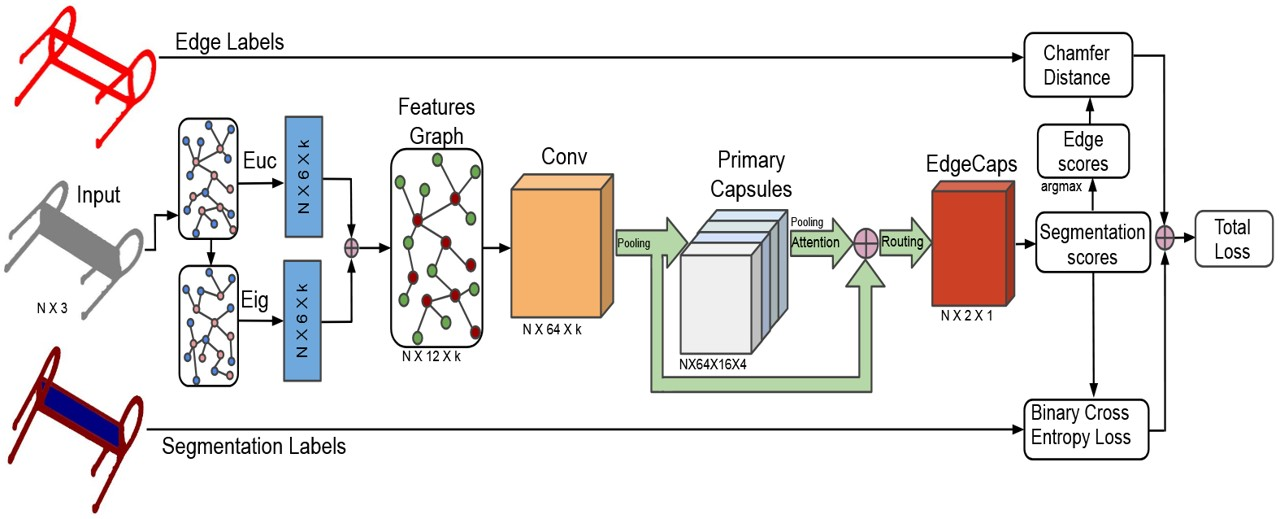
\includegraphics[width=0.95\textwidth]{Others/bazazian_edcnet_2021.jpg}
    \bicaption{基于胶囊网络的边缘检测方法 EDC-Net~\cite{bazazian_edcnet_2021}。}{EDC-Net: Capsule network-based method for edge detection~\cite{bazazian_edcnet_2021}.}
    \label{fig:bazazian_edcnet_2021}
\end{figure}
针对特征空间层级关系的建模，Bazazian 等人提出的 EDC-Net~\cite{bazazian_edcnet_2021} 引入了胶囊网络（Capsule Network），如图~\ref{fig:bazazian_edcnet_2021} 所示。该方法首先将局部邻域编码为几何描述符，利用胶囊层独特的动态路由机制来捕捉特征的空间分布结构，从而将点稳健地分类为非边缘或锐利边缘，减少了对人工参数的依赖。此外，针对输入形式的不同，Guerrero 等人的 PCPNet~\cite{guerrero_pcpnet_2018} 专注于局部几何属性的估计，它以多尺度的点云局部图块（Patches）作为输入，通过共享权重的 MLP 学习局部形状特征，不仅能估计法向量和曲率，也能用于特征点的分类。Jiao 等人的 MSL-Net~\cite{jiao_mslnet_2024} 则提出了一种轻量级的多尺度局域网络，通过在不同半径下聚合局部邻域信息增强特征表达，旨在解决大规模点云场景下边缘提取的实时性问题。

为了更有效地利用局部几何信息，Himeur 等人提出的 PCEDNet~\cite{himeur_pcednet_2022} 和 Bode 等人提出的 BoundED~\cite{bode_bounded_2023} 采用了基于多尺度局部特征描述符的策略。这类方法首先计算点云的多尺度几何属性（如曲率、法向量分布等），然后将这些描述符输入 MLP 进行特征融合与分类。研究表明，通过神经网络学习局部描述符的非线性组合，可以显著提升边缘检测的精度。然而，由于边缘和角点在局部邻域内的几何特征极具相似性，现有方法仍未运用于角点的检测，无法证明其有效性。

除了将被检测任务视为逐点分类问题，部分研究将其重构为回归问题或采用不同的数据表征。Yu 等人提出的 EC-Net~\cite{yu_ecnet_2018}不直接进行二分类，而是学习预测每个点到最近边缘的距离场（Distance Field）。通过回归距离值为零的等值线，EC-Net 能够以亚像素级的精度恢复出锐利的边缘曲线，尤其在处理倒角特征时表现优异。类似的，Matveev 等人的 DEFs~\cite{matveev_def_2022} 采用了一种隐式场回归的策略。该网络训练模型回归每个查询点到最近边缘曲线的距离以及特征点的坐标残差，随后通过后处理算法重建高精度的连续边缘线。

\begin{figure}[htbp]
    \centering
    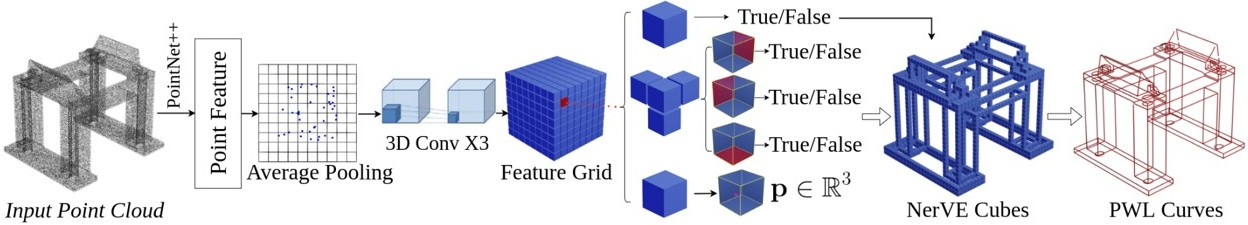
\includegraphics[width=1.0\textwidth]{Others/zhu_nerve_2023.jpg}
    \bicaption{基于体素网格的边缘检测方法 NerVE~\cite{zhu_nerve_2023}。}{NerVE: Voxel-based edge detection method~\cite{zhu_nerve_2023}.}
    \label{fig:zhu_nerve_2023}
\end{figure}
在数据表征方面，Zhu 等人提出的 NerVE~\cite{zhu_nerve_2023} （如图~\ref{fig:zhu_nerve_2023} 所示）针对无序点云难以进行常规卷积的问题，将点云转化为规则的体素（Voxel）网格。该方法利用稀疏三维卷积神经网络提取体素特征，并在体素内进一步进行节点分类，在保持结构化感知的同时实现了对尖锐几何特征的有效检测。Hu 等人的 JSENet~\cite{hu_jsenet_2020} 则将任务扩展为三维语义边缘检测，采用双流全卷积架构，一支流负责语义分割，另一支流专注边缘检测，通过特征交互模块融合两者的信息，从而在提取几何边缘的同时赋予其语义类别属性。这种方法的检测结果不仅具有几何准确性，还能提供丰富的语义信息，但其处理效率较低，在大规模点云场景下的适应性有待提升。

总体而言，目前的学习型方法主要集中在边缘特征提取上，且效果显著，但针对角点检测的研究相对匮乏。PCEDNet 和 BoundED 等方法证明了通过神经网络学习局部几何描述符在边缘检测上的有效性。基于此，本文延续并改进这一技术路线：针对角点和边缘难以区分的难点，本文对计算特征描述符进行针对性的设计，提出了能够有效辨识角点的新型几何特征，并采用基于 MLP 的层次化网络结构来学习这些特征，从而实现对面、边缘和角点三类特征的高精度同步检测。

\subsection{机器人抓取规划研究现状}
机器人抓取规划主要可以分为抓取构型（Grasp Configuration）规划和抓取质量评估两个方面。这两部分都包括基于分析和数据驱动的方法。
\subsubsection{抓取构型规划}
机器人抓取规划方法通常可分为基于模型（Model-based）和基于学习（Learning-based）的方法。基于模型的方法依赖于物体的几何信息和物理规则来生成抓取构型，这类方法进一步可分为两种主要策略：图元拟合（Primitive Fitting）和表面分割（Surface Segmentation）。

图元拟合策略使用基本的几何图元（如圆柱体、球体、方块等）来近似物体，从而简化抓取合成过程~\cite{goldfeder_grasp_2007}。Miller 等人提出了 GraspIt! 仿真器~\cite{miller_automatic_2003,miller_graspit_2021}，通过将复杂物体分解为一组简单的几何原语来快速生成抓取假设。Chen 等人~\cite{chen_category_2022} 利用词嵌入（Word Embeddings）来量化已知模型类别与真实物体之间的语义相似度，从而实现新物体与数据库模型的匹配。虽然图元近似降低了计算复杂度，但它往往丢失了物体的局部细节几何信息，导致生成的抓取难以适应具有丰富几何特征的复杂物体。
\begin{figure}[htbp]
    \centering
    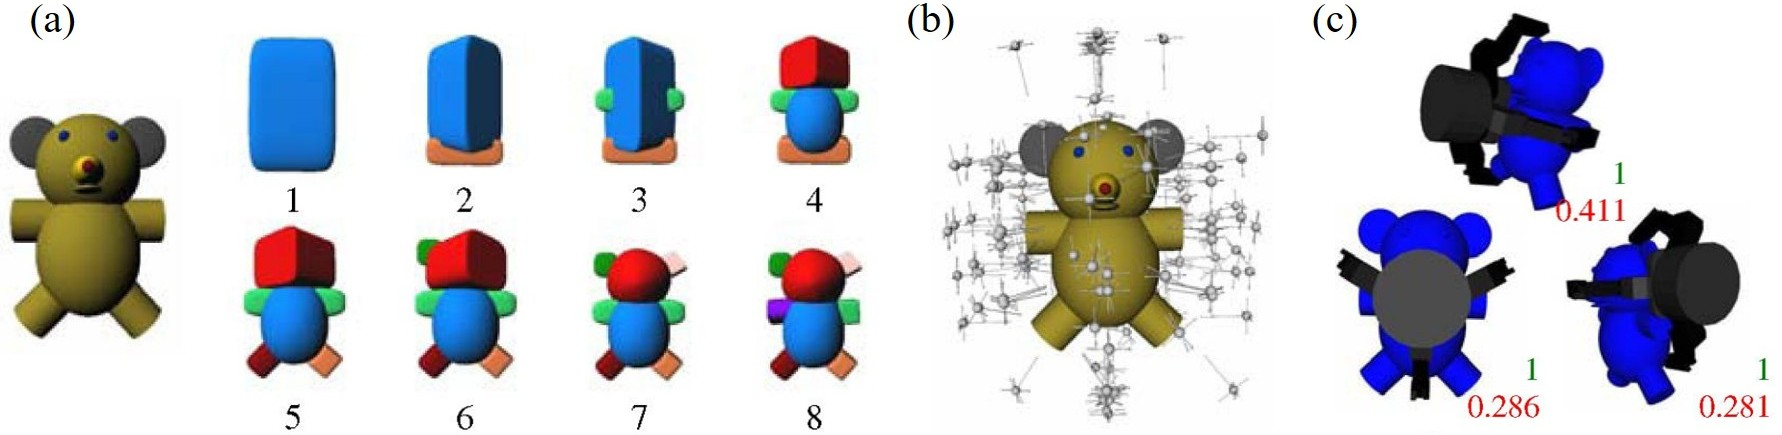
\includegraphics[width=0.95\textwidth]{Others/goldfeder_grasp_2007.jpg}
    \bicaption{基于图元拟合的抓取规划方法~\cite{goldfeder_grasp_2007}：(a) 图元拟合过程；(b) 抓取构型生成；(c) 抓取质量评估。}{Grasp planning method based on primitive fitting~\cite{goldfeder_grasp_2007}: (a) Primitive fitting process; (b) Grasp configuration generation; (c) Grasp evaluation.}
    \label{fig:goldfeder_grasp_2007}
\end{figure}

表面分割策略则致力于识别有意义的表面区域以指导抓取生成。Harada 等人~\cite{harada_grasp_2011} 针对软指尖手爪，根据接触软度对三角网格进行聚类，规划出适应物体局部曲率的抓取。Wan 等人~\cite{wan_planning_2021} 引入了叠加分割（Superimposed Segmentation）技术，根据表面法向量将每个三角形分割为具有受控重叠和厚度的多个面片。然而，为了确保力封闭的稳定性，这类方法通常显式地剔除边缘和角点附近的区域，避免在曲率突变处建立接触~\cite{wan_planning_2021, miller_graspit_2021}。这种“面接触优先”的策略虽然提高了抓取的保守稳定性，却极大限制了抓取构型在物体表面的分布，导致灵活性不足。
\begin{figure}[htbp]
    \centering
    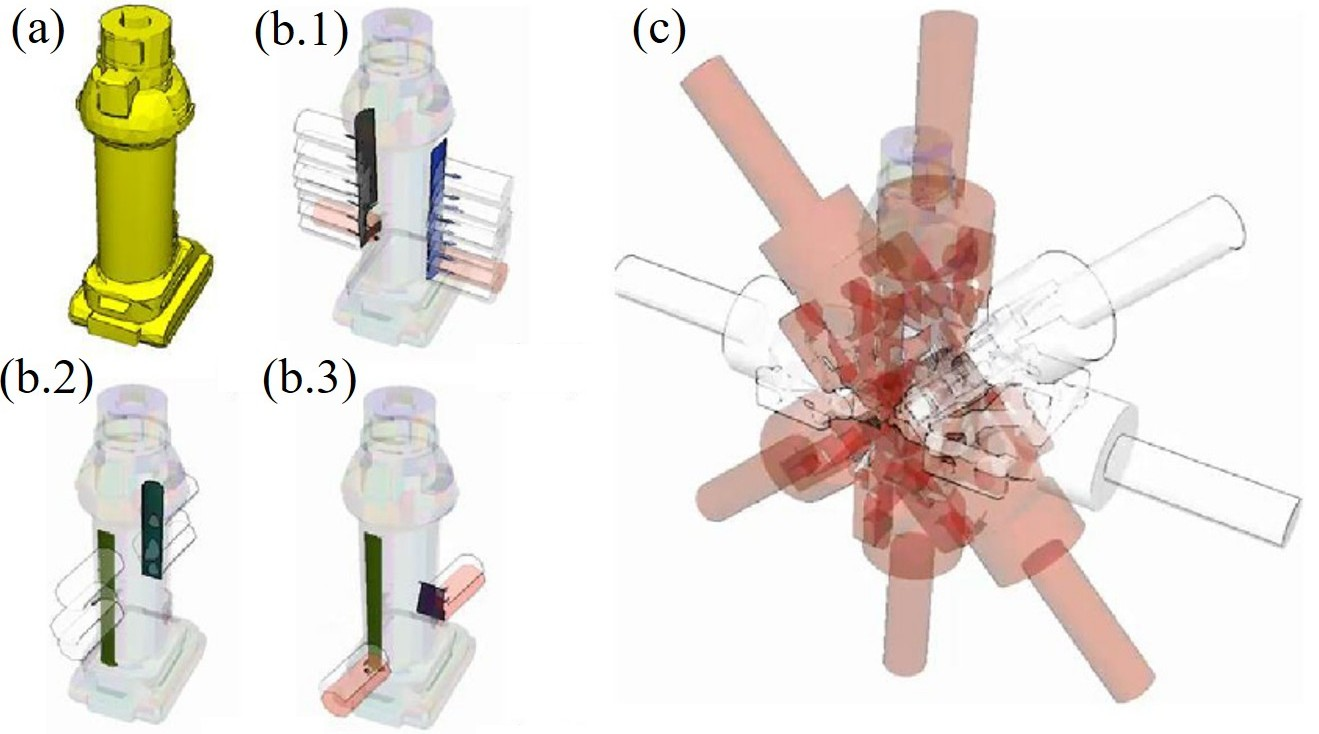
\includegraphics[width=0.6\textwidth]{Others/wan_planning_2021.jpg}
    \bicaption{基于表面分割的抓取规划方法~\cite{wan_planning_2021}：(a)物体模型；(b.1-3)表面分割结果；(c)抓取构型生成。}{Grasp planning method based on surface segmentation~\cite{wan_planning_2021}: (a) Object model; (b.1-3) Surface segmentation results; (c) Grasp configuration generation.}
    \label{fig:wan_planning_2021}
\end{figure}

另一方面，基于学习的方法利用神经网络和数据驱动技术来增强抓取的泛化能力。Mahler 等人提出的 Dex-Net~\cite{mahler_dexnet_2017,mahler_learning_2019} 系列构建了大规模的合成抓取数据集，训练卷积神经网络（GQ-CNN）直接从深度图像中预测平面抓取的成功率。Mousavian 等人~\cite{mousavian_graspnet_2019} 则提出了 6-DOF GraspNet，通过基于变分自编码器（VAE）的框架生成多样化的6自由度抓取构型。该方法利用抓取评价或精炼网络对候选进行评分并迭代优化，以提高抓取的稳定性与可执行性；最终结合碰撞检测等几何约束过滤不可行抓取，实现对复杂物体的多样化6D抓取构型生成。
\begin{figure}[htbp]
    \centering
    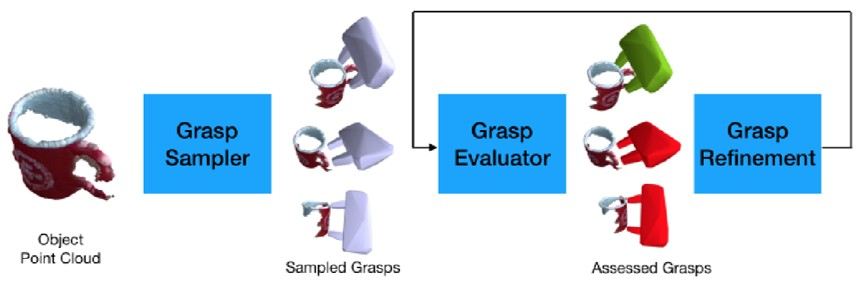
\includegraphics[width=0.9\textwidth]{Others/mousavian_graspnet_2019.jpg}
    \bicaption{基于变分自编码器的6-DOF抓取生成方法~\cite{mousavian_graspnet_2019}。}{6-DOF grasp generation method based on variational autoencoder~\cite{mousavian_graspnet_2019}.}
    \label{fig:mousavian_graspnet_2019}
\end{figure}

尽管这些方法在未见过物体上表现出色，但其训练数据通常是基于传统解析指标（如 GraspIt! 中的能量函数）生成的~\cite{fang_graspnet1billion_2020}。因此，数据驱动模型倾向于继承“排斥边缘”的偏见，将边缘和角点视为噪声或不稳定区域，从而难以生成涉及这些尖锐特征的多样化抓取~\cite{mahler_learning_2019, cao_efficient_2023}。
本文提出的方法打破了这一局限，引入软接触模型，将潜在的稳定接触扩展到边缘和角点。通过开发包含边缘和角点接触的抓取规划算法，旨在显著增加抓取分布的覆盖率和灵活性。

\subsubsection{抓取质量评估}
为了评估抓取候选的可行性和质量，研究者提出了多种抓取评价标准。最常用的解析指标是抓取稳定性，通常通过力封闭（Force Closure）或形封闭（Form Closure）条件进行评估~\cite{bicchi_robotic_2000}。解析方法通过评估旋量空间覆盖率（Wrench Space Coverage）、抗扭矩能力或最小力需求来确定抓取的可靠性。Ferrari 和 Canny~\cite{ferrari_planning_1992} 提出了经典的 $\epsilon$ 指标，通过计算抓取矩阵在旋量空间中张成的最大球半径（$L_2$ 范数）或最大多胞体体积（$L_1$ / $L_\infty$ 范数）来量化抓取抵抗外部扰动的能力。然而，这些解析指标通常假设刚性接触，对于边缘和角点这类理论上接触面积为零的区域，往往给出极低的稳定性评分。

相比之下，数据驱动方法通常训练模型直接从视觉或几何输入预测抓取质量评分。Ten Pas 等人提出的 GPD（Grasp Pose Detection）算法~\cite{tenpas_grasp_2017} 则直接在三维点云中采样候选抓取，并对物体点云进行投影，利用CNN网络评估其抓取质量。Liang 等人则对 GPD 的抓取质量评估网络进行了改进，提出了基于 PointNet++ 的 PointNetGPD~\cite{liang_pointnetgpd_2019}，通过引入多尺度特征融合和注意力机制来提升评估的准确性和鲁棒性，并且无需对点云进行投影。
\begin{figure}[htbp]
    \centering
    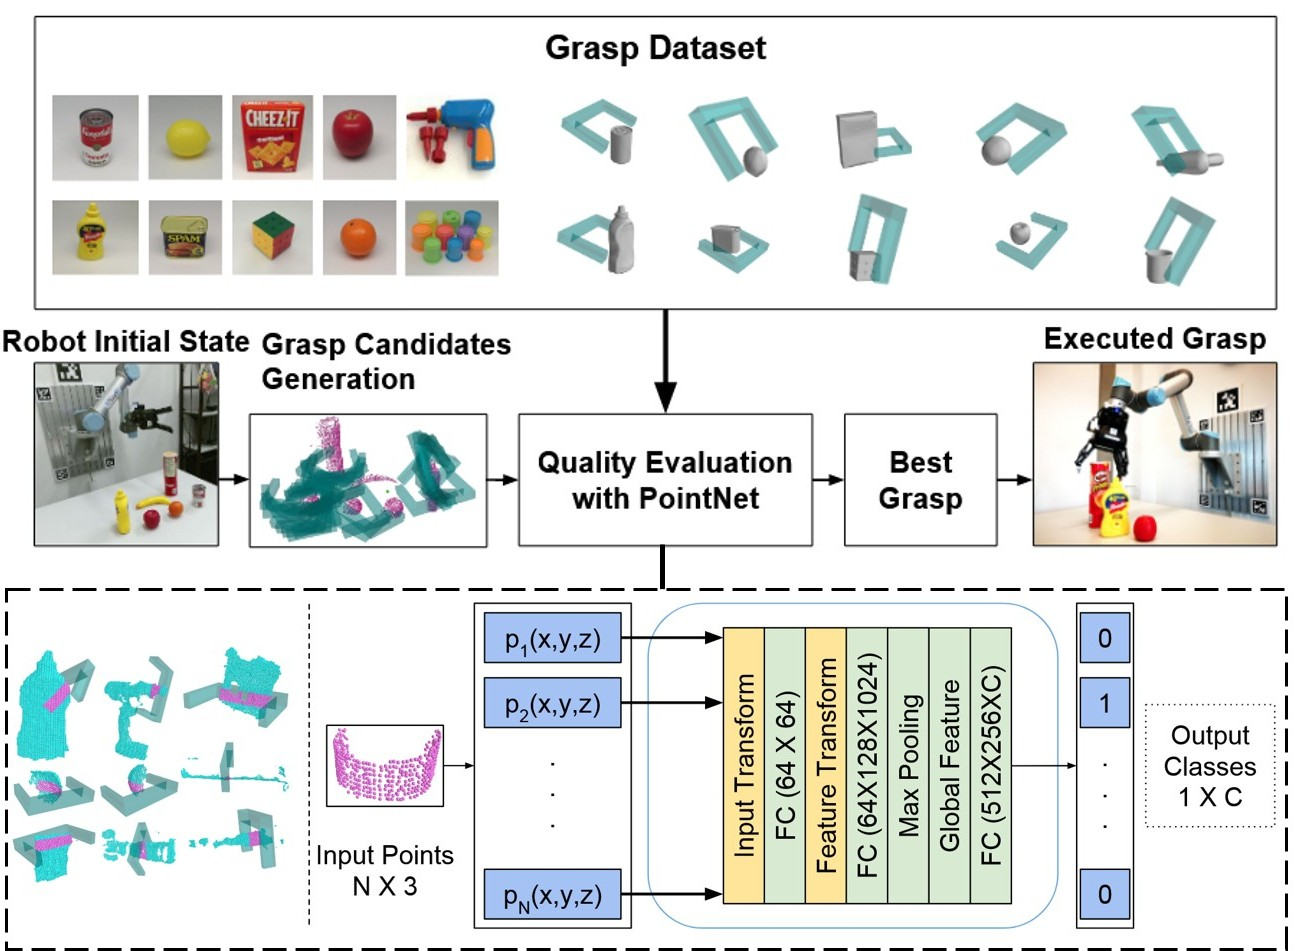
\includegraphics[width=0.85\textwidth]{Others/liang_pointnetgpd_2019.jpg}
    \bicaption{基于深度学习的抓取质量评估方法 PointNetGPD~\cite{liang_pointnetgpd_2019}。}{PointNetGPD: Grasp Pose Detection method based on deep learning~\cite{liang_pointnetgpd_2019}.}
    \label{fig:liang_pointnetgpd_2019}
\end{figure}

近期，Yu 等人~\cite{yu_mtgrasp_2025} 和 Cao 等人~\cite{cao_efficient_2023} 引入了更先进的深度网络架构来捕捉抓取区域的全局上下文信息，进一步提升了评估的准确性。虽然这些学习模型可能缺乏如力封闭等形式化保证，但它们在非结构化和实时环境中表现出了卓越的适应性。此外，一些混合方法结合了解析指标与数据驱动模型，以增强泛化能力和鲁棒性~\cite{kopicki_learning_2014}。

值得注意的是，现有的大多数评价指标主要关注单个抓取构型的成功率或稳定性，而缺乏对规划器生成的抓取解集在物体表面空间分布情况的量化评估。针对这一问题，本文引入了一种基于统计熵的指标，用于量化抓取构型的分布均匀性，并作为抓取灵活性的代理指标。该指标能够对不同规划器在抓取灵活性方面进行定量且直观的比较，而不受其选择接触区域优先级的差异影响。

\section{本文主要研究内容}
\label{sec:contribution}

针对物体几何特征检测中存在的角点识别困难、检测精度不足的问题，以及机器人抓取规划中因过分依赖面接触而导致的抓取灵活性受限问题，本文开展了系统性的研究工作。本文的核心目标是建立一套从高精度几何感知到灵活多模式抓取规划的完整技术方案。本文的主要研究内容包括以下两个方面：

第一，本文提出了一种基于多尺度局部特征融合的点云边缘与角点检测流程框架（NECDNet）。针对现有方法在角点检测上的缺失，该研究设计了一套包含曲率、投影距离、法向分布等六个维度的解析特征描述符，专门用于捕捉稀疏且模糊的角点信号。通过构建多尺度邻域特征矩阵作为输入，并设计基于多层感知机（Multi Layer Perceptron, MLP）的层次化分类网络，该方法实现了对点云中面、边缘、角点三类特征的高精度端到端识别。如图~\ref{fig:necdnet_result} 所示，较其余方法，该网络不仅保持了边缘检测的高性能，更显著提升了角点检测的准确率。

\begin{figure}[htbp]
    \centering
    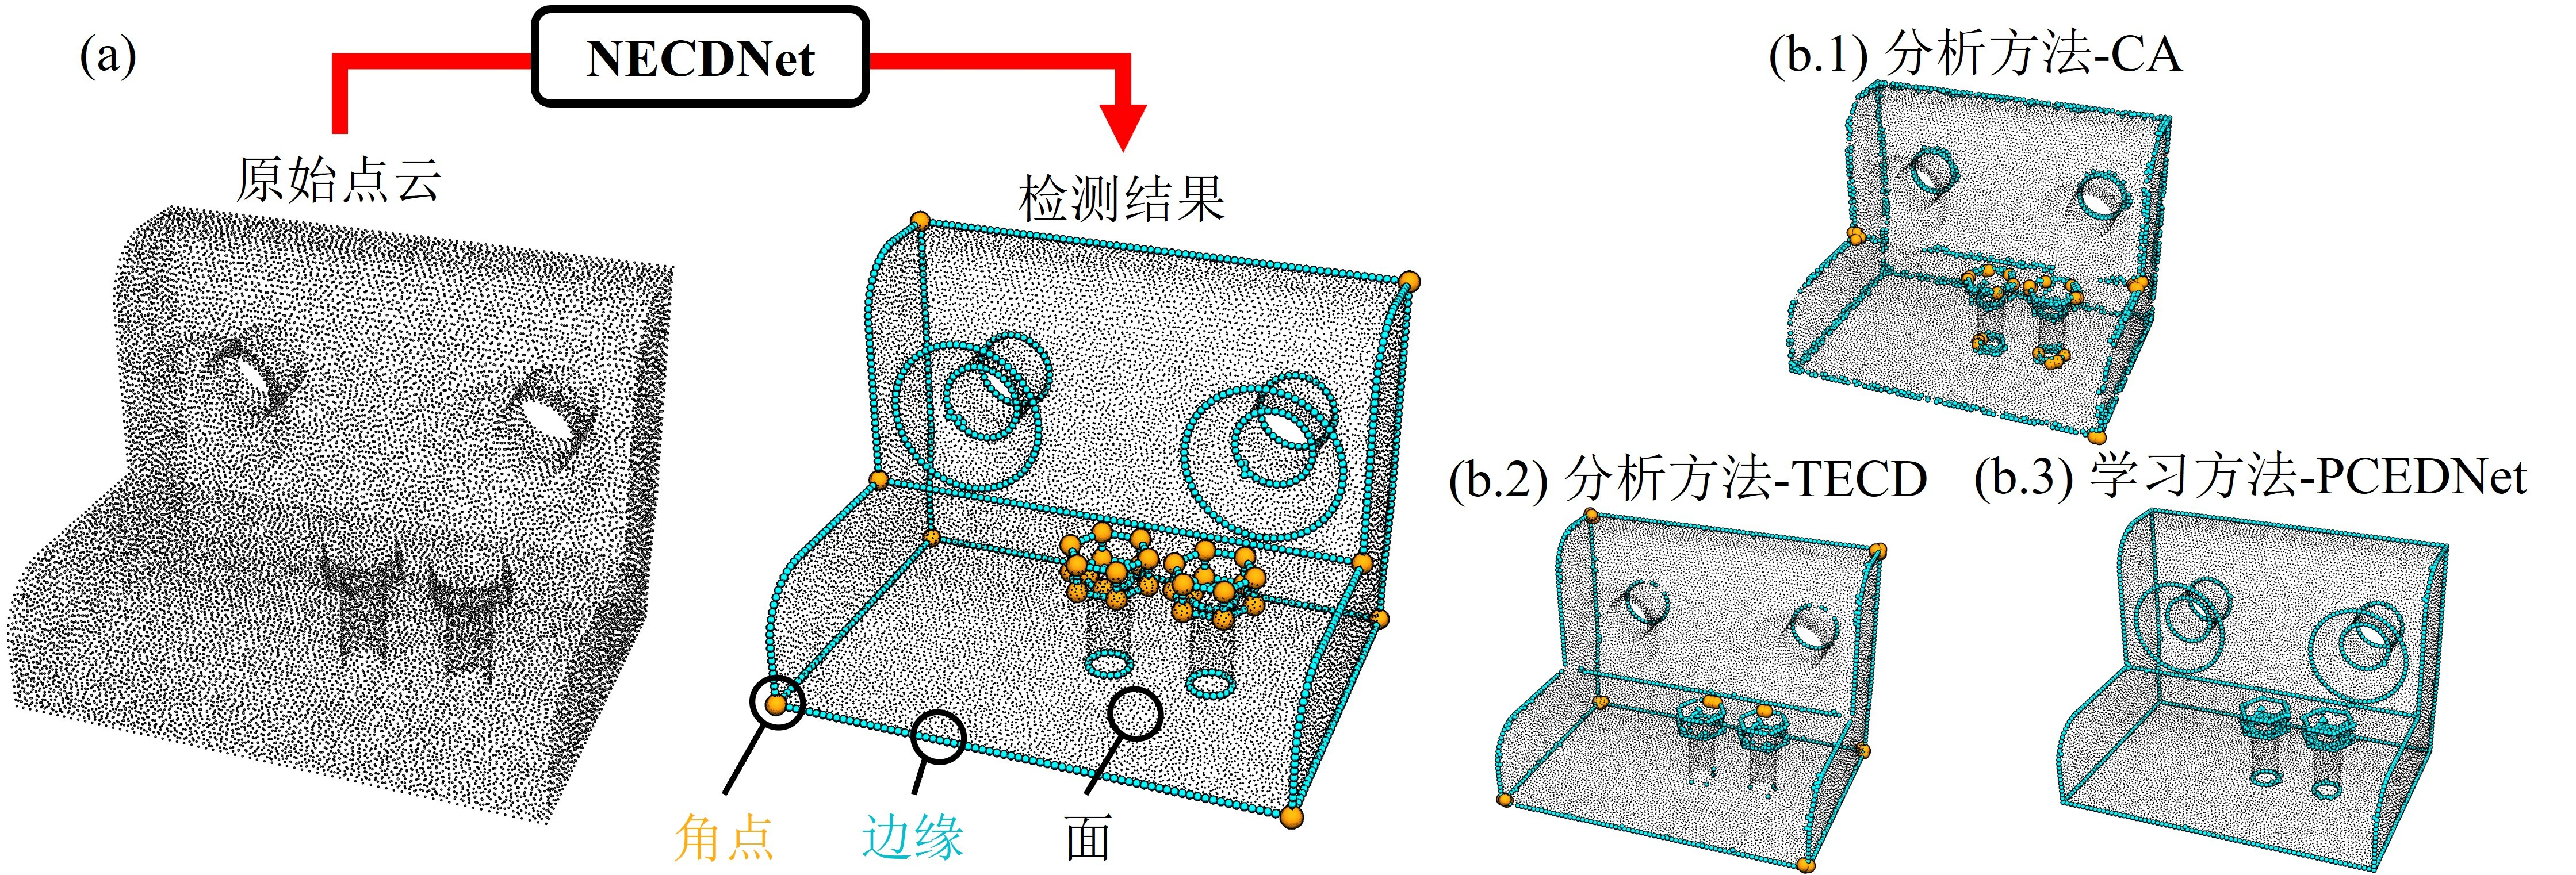
\includegraphics[width=1.0\textwidth]{NECDNet/teaser.jpg}
    \bicaption{不同几何特征检测方法结果对比：(a) NECDNet；(b.1-3) CA~\cite{gumhold_feature_2001}, TECD~\cite{ahmed_edge_2018}, PCEDNet~\cite{himeur_pcednet_2022}。}{Comparison of geometric feature detection results: (a) NECDNet; (b.1-3) CA~\cite{gumhold_feature_2001}, TECD~\cite{ahmed_edge_2018}, PCEDNet~\cite{himeur_pcednet_2022}.}
    \label{fig:necdnet_result}
\end{figure}

其中，为了解决深度学习方法在几何特征检测领域面临的训练数据匮乏问题，本文构建了 ABC-Corner 基准数据集。该数据集从大规模 CAD 模型库 ABC 数据集中精选了 1000 个具有丰富几何细节的代表性模型。通过结合基于几何规则的自动初筛算法与人工精细交互修正的标注流程，生成了包含面、边缘、角点三类高精度标签的点云数据。该数据集填补了领域内缺乏专门针对角点检测的大规模公开数据集的空白，为后续的数据驱动算法研究提供了可靠的基准。

第二，本文提出了一种考虑边缘和角点接触的六自由度机器人抓取规划算法。该算法突破了传统面接触优先的规划范式，将边缘和角点纳入可行的接触候选区域。算法利用提取的几何特征进行类别感知的均衡采样，并针对面、边、角三种不同特征分别设计了圆柱形、扇形和圆锥形接触检测器，以高效搜索潜在的对指抓取配对。通过引入基于离散化的软指接触模型，实现了对边缘和角点接触稳定性的有效评估。此外，本文还首次引入了抓取分布统计指标来量化评估抓取规划的灵活性。如图~\ref{fig:fbgrasp_result} 展示了该算法生成的抓取构型，实验结果证明，该方法在正四面体、非对称曲面等复杂物体上实现了极高的抓取成功率和空间覆盖率。

\begin{figure}[htbp]
    \centering
    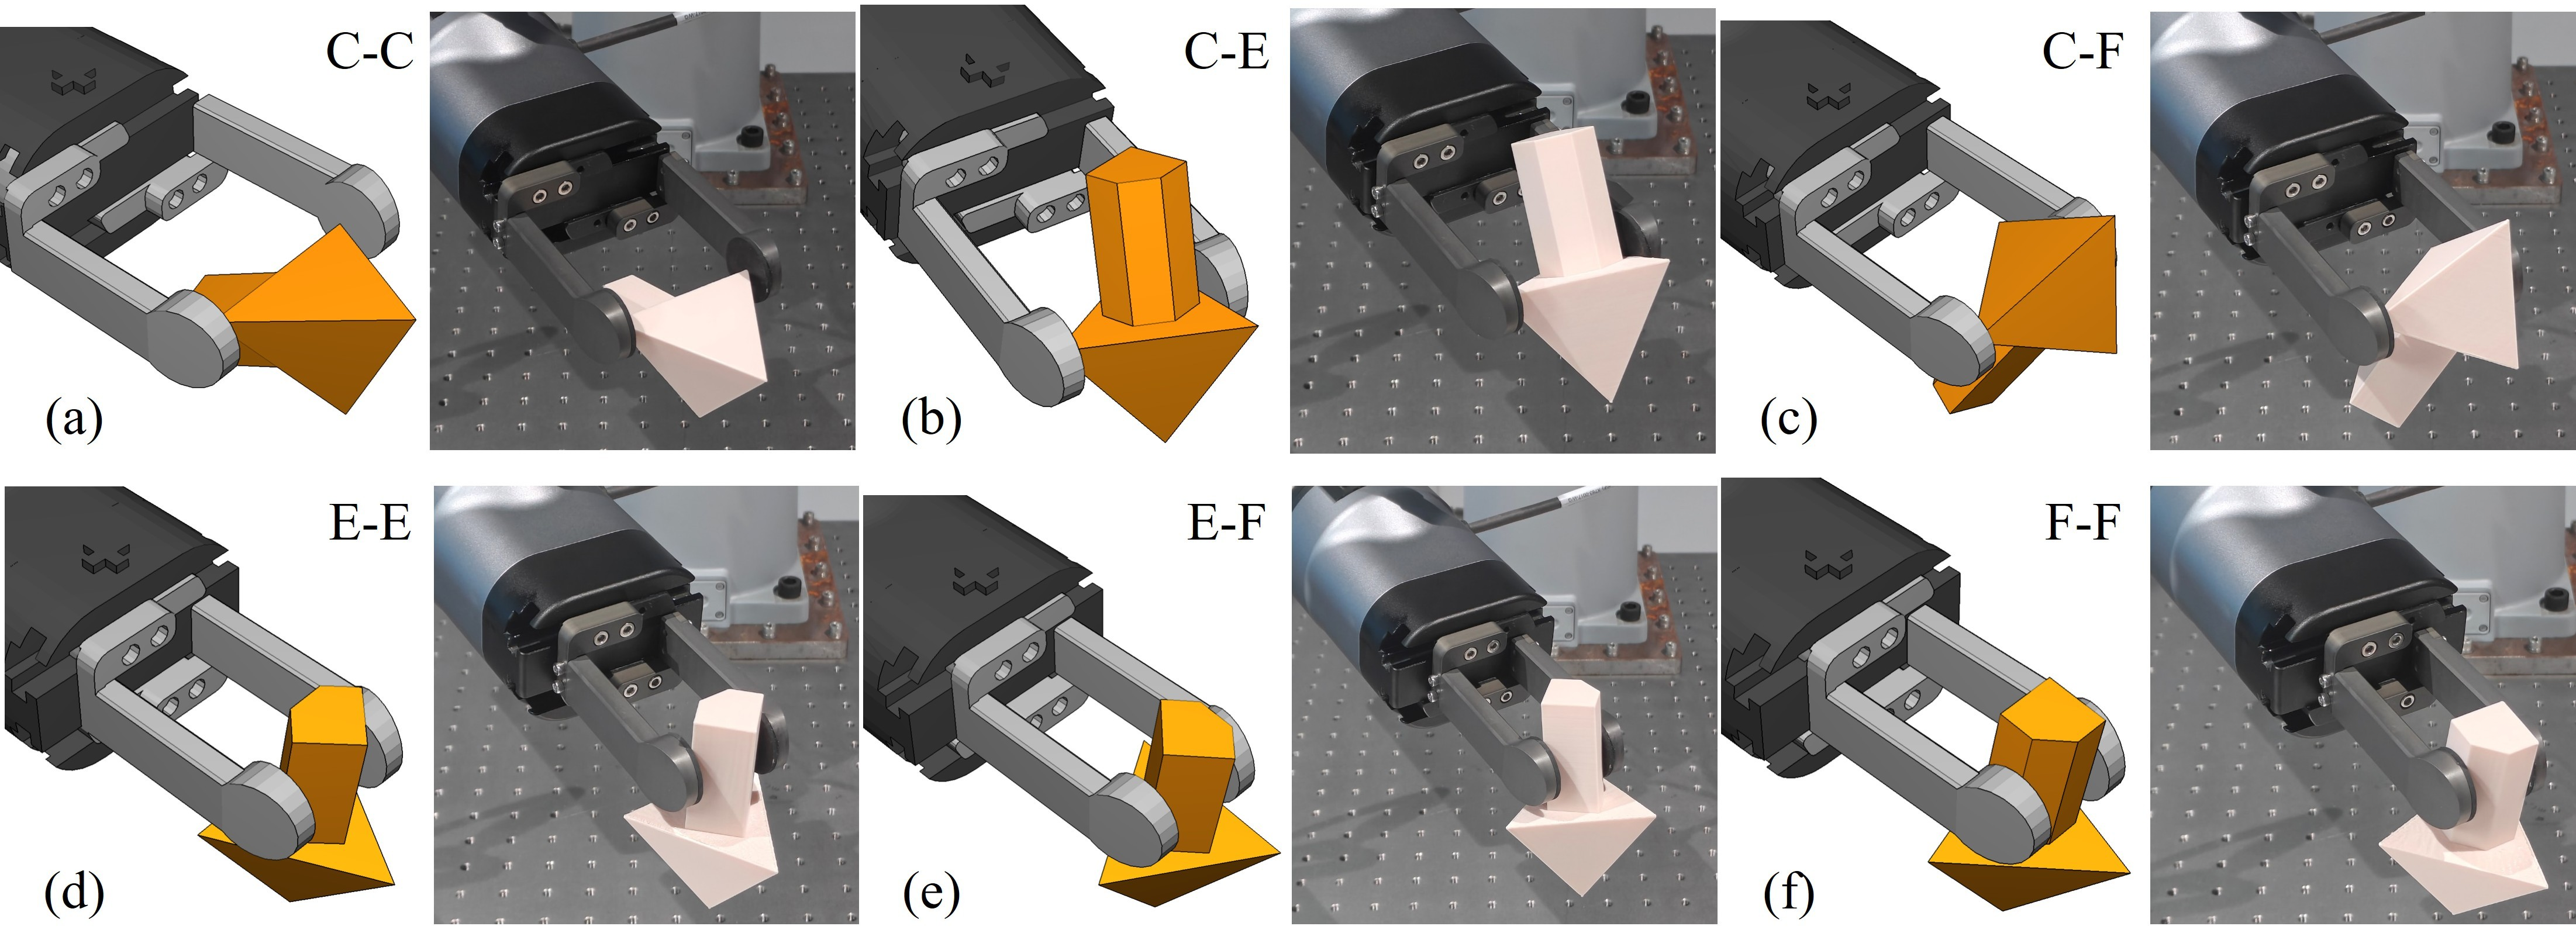
\includegraphics[width=1.0\textwidth]{FBGrasp/teaser.jpg}
    \bicaption{基于物体几何特征的抓取规划结果展示：(a-f) 针对三种几何特征实现的六种抓取构型，依次为：角-角，角-边，角-面，边-边，边-面，面-面。}{Grasp planning results based on object geometric features: (a-f) Six grasp configurations for three geometric features, including C-C, C-E, C-F, E-E, E-F, and F-F.}
    \label{fig:fbgrasp_result}
\end{figure}

综上所述，本文的主要创新点可以归纳为以下三个方面：

（1）提出了一种融合显式几何描述符与数据驱动的基于物体点云的几何特征检测网络（NECDNet）。 通过引入多尺度显式几何特征描述符，解决了纯数据驱动方法在稀疏角点检测上的特征模糊问题，实现了对面、边缘和角点的高精度同步检测。

（2）构建了包含高精度角点标注的大规模点云几何特征数据集（ABC-Corner）。针对现有数据集缺乏角点标注的问题，建立了一套半自动化的精细标注流程，为几何特征检测领域提供了高质量的数据基准。

（3）提出了一种基于软接触模型并融合边缘与角点接触的抓取规划算法。该算法突破了传统面接触优先假设，针对不同几何特征设计了专门的抓取构型检测策略，并引入抓取分布统计指标以量化评估抓取灵活性，同时采用软接触模型进行抓取稳定性评估，从而显著提升了机器人在复杂物体抓取任务中的灵活性和空间覆盖率。

\section{论文组织结构}
\label{sec:structure}

本文共分为六章，各章节的具体内容安排如下：

第一章为绪论，主要阐明点云几何特征检测与机器人抓取规划的研究背景和工程意义，系统梳理国内外相关研究进展，分析现有方法在角点检测精度与抓取灵活性方面的不足，并据此明确本文的研究目标、技术路线与主要创新点。

第二章围绕点云几何特征检测方法展开，重点介绍 NECDNet 的整体框架与实现过程，包括多尺度 $k$ 近邻邻域构建、六维显式几何描述符设计以及基于多层感知机的层次化分类结构。

第三章在上述方法基础上开展实验评估，首先给出 ABC-Corner 数据集的构建流程，为后续实验提供数据基础。之后通过与主流方法的定性和定量对比验证 NECDNet 在边缘与角点检测任务中的性能优势，并结合消融实验进一步分析特征维度、网络模块及法向量估计精度对结果的影响。

第四章进一步面向机器人抓取规划问题，提出一种考虑边缘与角点接触的六自由度抓取规划方法，系统介绍类别感知采样、面/边/角接触检测器设计、接触对构建与软接触稳定性评估等关键环节，形成从几何特征到抓取构型生成的完整流程。

第五章对所提抓取规划方法进行实验验证，分别从仿真与真实物理实验两个层面评估其性能，并通过抓取分布统计指标、抓取成功率指标与对比方法进行综合分析，验证方法在复杂几何物体上的有效性与实用性。最后分析了算法计算效率。

第六章对全文工作进行总结，归纳本文在物体几何特征检测与机器人抓取规划两方面的主要贡献，客观讨论当前方法的局限，并结合机器人操作场景的发展需求给出后续研究方向与改进思路。











